\documentclass[11pt,a4paper]{report}

\usepackage[utf8]{inputenc}
\usepackage{titling}
\usepackage[german]{babel}
\usepackage[T1]{fontenc}
\usepackage{amsmath}
\usepackage{amsfonts}
\usepackage{amssymb}
\usepackage[left=3cm,right=2cm,top=2.5cm,bottom=2cm]{geometry}
\usepackage{graphicx}
\usepackage{fancyhdr}
\usepackage{color}
\usepackage[
colorlinks=true,
urlcolor=blue,
linkcolor=black
]{hyperref}
\pagestyle{fancy}

\lhead{Sina Opitz}
\chead{ak18b}
\rhead{13.01.2019}

\lfoot{}
\cfoot{\thepage}
\rfoot{}

\renewcommand{\headrulewidth}{0.4pt}
\renewcommand{\footrulewidth}{0.4pt}

\begin{document}
	\begin{titlepage}
		
		\pretitle{
			\vskip -3em
			\begin{figure}[h]
				\begin{center}
					
\includegraphics[scale=0.55]{Logo.png}
				\end{center}
			\end{figure}
			\begin{center}
				\vskip -2em
				\large{Wintersemester 2018/19\\Softwaretechnikpraktikum} \vskip 9em
				\rule{5in}{0.4pt}\par \vskip 0.5em
			}
			\posttitle{\par\rule{5in}{0.4pt} \vskip 4em
				\Large Gruppe: ak18b \vskip 1.5em
				\normalsize Betreuer: Benjamin Lucas Friedland, Michael Fritz\vskip 1em
				\normalsize Gruppenmitglieder: Alexander Zwisler, Leon Kamuf, Leon Rudolph, Maurice Eisenblätter, Maximilian Gläfcke, Robin Seidel, Sina Opitz, Steve Woywod
		\end{center}}
		
		\title{\textbf{\Huge App zur Inventarisierung von Unternehmenswerten}\vskip 0.5em \huge Benutzerhandbuch}
		\date{}
		\maketitle
	\end{titlepage}
	\setcounter{secnumdepth}{4}
	\setcounter{tocdepth}{4}
	\tableofcontents
	\thispagestyle{empty}
	\newpage
	\setcounter{page}{1}
	\renewcommand\thesection{\arabic{section}}
	
	\section{Allgemeine Informationen}
	\subsection{Einführung}
Herzlich Willkommen!
\\~\\
Dieses Handbuch hilft Ihnen die Inventarisierungsapp optimal zu nutzen.\\
Wir wünschen Ihnen viel Freude bei der Nutzung!\\
Optimiert wurde die Web-App für Google Chrome.
\\~\\
Änderungen vorbehalten\\
Version 1/11.03.19
	\subsection{Ihre Vorteile}
	\begin{itemize}
		\item intuitive Benutzeroberfläche
		\item für jedes Unternehmen geeignet
		\item vollständige digitale Inventarisierung
		\item übersichtliche Darstellung aller Gegenstände
		\item Erstellen von Benutzerrollen zur Sicherung aller Gegenstände
		\item Gruppieren der Gegenstände nach Typen
	\end{itemize}
	\section{Erste Schritte}
	\textbf{Die App läuft vollständig im Browser. Es ist also keine Installation auf Ihrem Rechner nötig!}\\
	Empfohlener Browser: Google Chrome
	
	\begin{itemize}
		\item Rufen Sie im Browser die App auf
		\item Loggen Sie sich mit Ihrem Benutzernamen und Passwort an
	\end{itemize}
	
	\section{Verwenden der Inventarisierungsapp}
	\subsection{Einen Objekttypen hinzufügen}
	
	\begin{itemize}
		\item[1.] Klicken Sie auf \glqq{}Objekttypen\grqq{}
		\item[2.] Klicken Sie auf \texttt{+} neben der Suchleiste
	\end{itemize}

	\begin{minipage}{0.5\linewidth}
	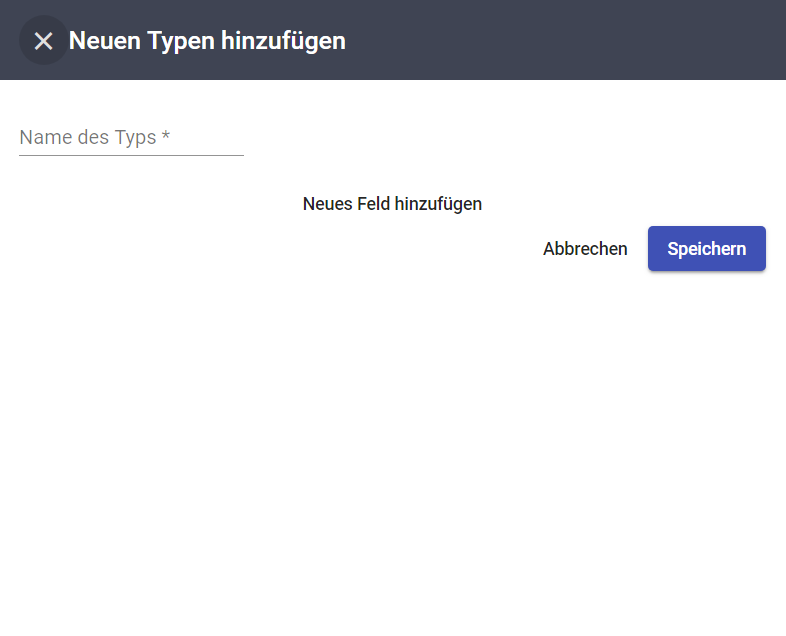
\includegraphics[width=\linewidth]{Objekttyp.png}
	\end{minipage}
	\hfill
	\begin{minipage}{0.4\linewidth}
	\begin{itemize}
		\item[3.] Wählen Sie einen Namen für Ihren Objekttypen
		\item[4.] Fügen Sie beliebig viele Felder hinzu
	\end{itemize}
	\end{minipage}\\

	\begin{minipage}{0.5\linewidth}
	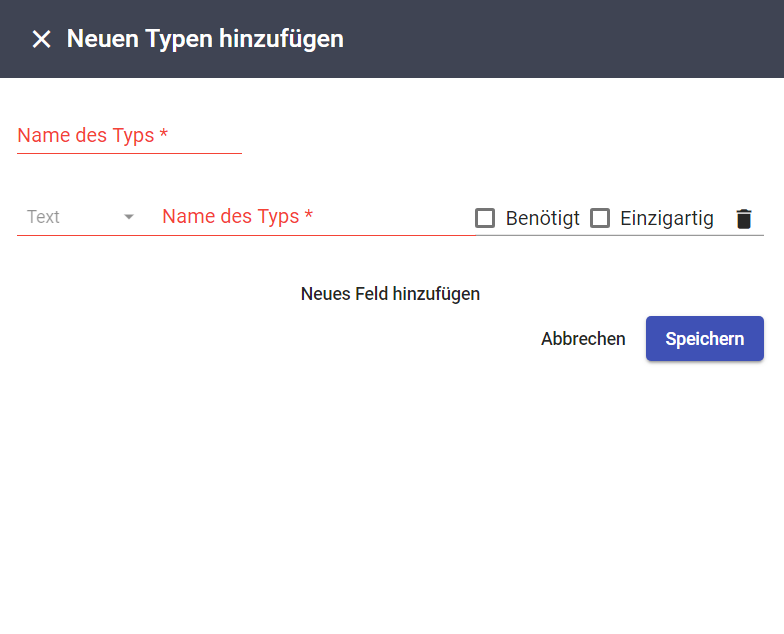
\includegraphics[width=\linewidth]{Objekttypadd.png}
	\end{minipage}
	\hfill
	\begin{minipage}{0.4\linewidth}
	\begin{itemize}
		\item[5.] Wählen Sie einen Datentypen
		\item[6.] Wählen Sie einen Namen für das Feld
		\item[7.] Entscheiden Sie, ob das Feld ein Pflichtfeld sein soll
		\item[8.] Entscheiden Sie, ob das Feld einzigartig sein soll
		\item[9.] Klicken Sie auf Speichern
	\end{itemize}
	\end{minipage}\\

	\subsection{Einen Objekttypen bearbeiten oder löschen}

	\begin{itemize}
		\item[1.] Klicken Sie auf \glqq{}Objekttypen\grqq{}
		\item[2.] Klicken Sie auf den Objekttypen, den Sie bearbeiten oder löschen wollen
	\end{itemize}

	\begin{minipage}{0.5\linewidth}
	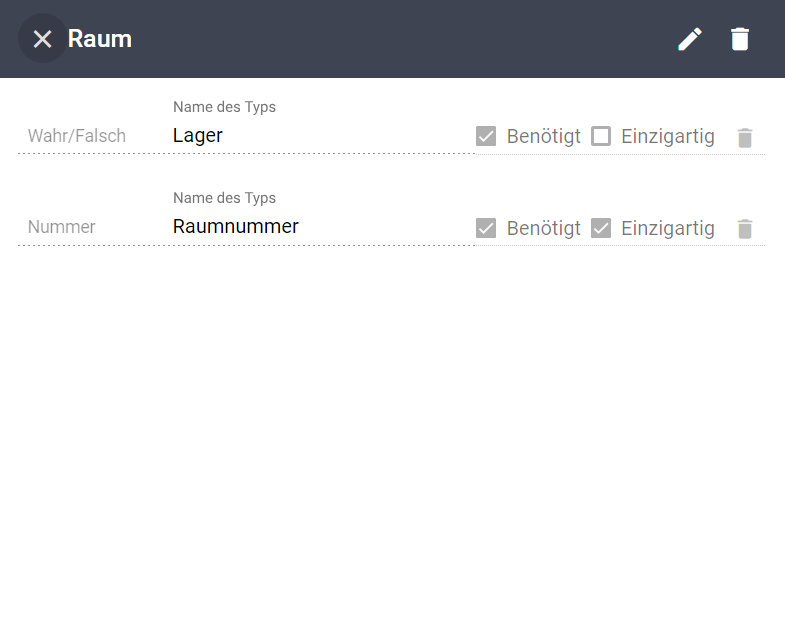
\includegraphics[width=\linewidth]{Objekttypedit.png}
	\end{minipage}
	\hfill
	\begin{minipage}{0.4\linewidth}
	\begin{itemize}
		\item[3.] Wählen Sie (1) aus, um die Objekttypen zu bearbeiten
		\item[4.] Wählen Sie (2) aus, um alle Objekttypen zu löschen\\
		ACHTUNG: Löschen der Objekttypen löscht auch deren Inhalte
	\end{itemize}
	\end{minipage}\\

	\begin{minipage}{0.5\linewidth}
	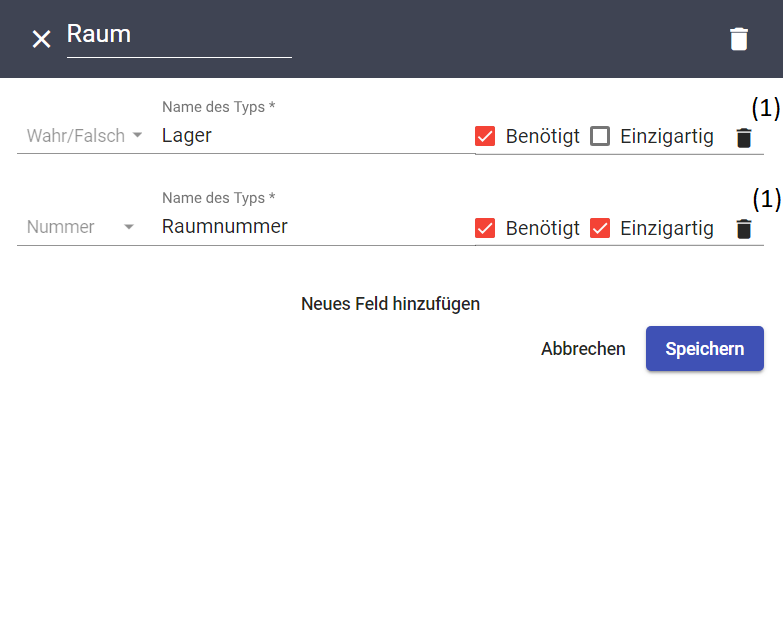
\includegraphics[width=\linewidth]{Objekttypedit2.png}
	\end{minipage}
	\hfill
	\begin{minipage}{0.4\linewidth}
	\begin{itemize}
		\item[5.] Bearbeiten Sie die Felder
		\item[6.] Wählen Sie (1) aus, um den Objekttypen zu löschen\\
		ACHTUNG: Löschen des Objekttypens löscht auch den Inhalt
	\end{itemize}
	\end{minipage}
\clearpage

	\subsection{Ein Objekt zu einem Objekttypen hinzufügen}

	\begin{itemize}
		\item[1.] Klicken Sie auf \glqq{}Inventar\grqq{}
		\item[2.] Klicken Sie auf \texttt{+} neben der Suchleiste
	\end{itemize}

	\begin{minipage}{0.5\linewidth}
	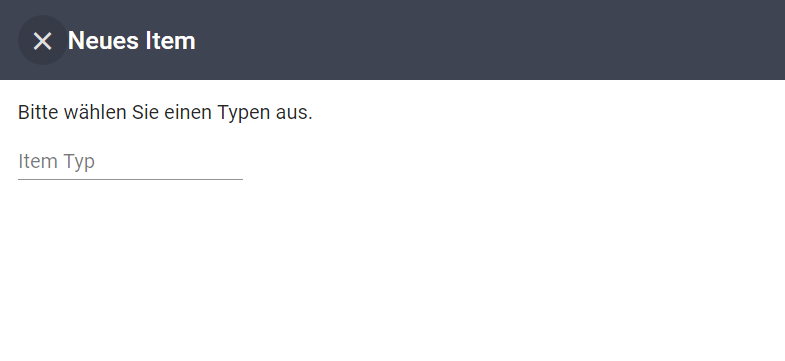
\includegraphics[width=\linewidth]{Inventar.png}
	\end{minipage}
	\hfill
	\begin{minipage}{0.4\linewidth}
	\begin{itemize}
		\item[3.] Wählen Sie aus, welchem Objekttyp ein Objekt hinzugefügt werden soll
	\end{itemize}
	\end{minipage}\\

	\begin{minipage}{0.5\linewidth}
	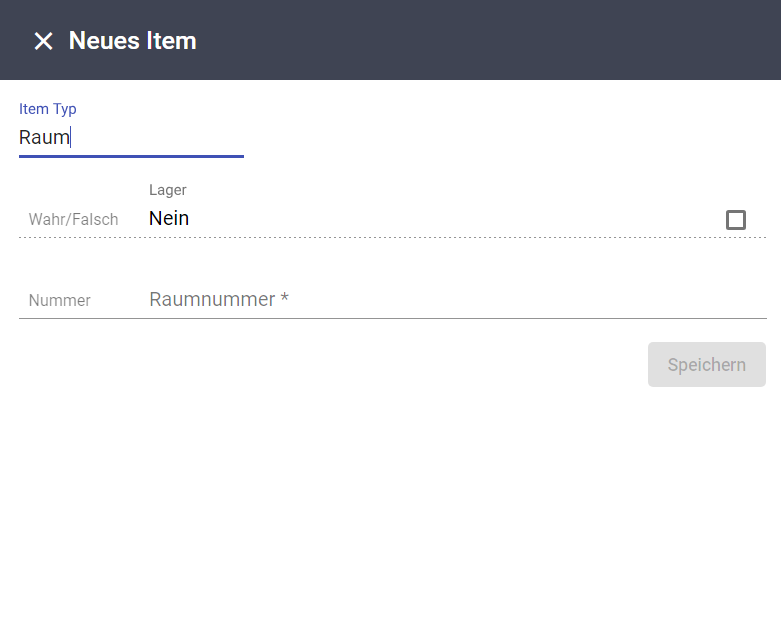
\includegraphics[width=\linewidth]{Inventar2.png}
\end{minipage}
\hfill
\begin{minipage}{0.4\linewidth}
	\begin{itemize}
		\item[4.] Füllen Sie die Felder aus\\
		Mit * markierte Felder sind Pflichtfelder
		\item[5.] Klicken Sie auf Speichern
	\end{itemize}
\end{minipage}\\

	\subsection{Ein Objekt bearbeiten oder löschen}

	\begin{itemize}
		\item[1.] Klicken Sie auf \glqq{}Inventar\grqq{}
		\item[2.] Klicken Sie auf das Objekt, das Sie bearbeiten oder löschen wollen
	\end{itemize}

	\begin{minipage}{0.5\linewidth}
	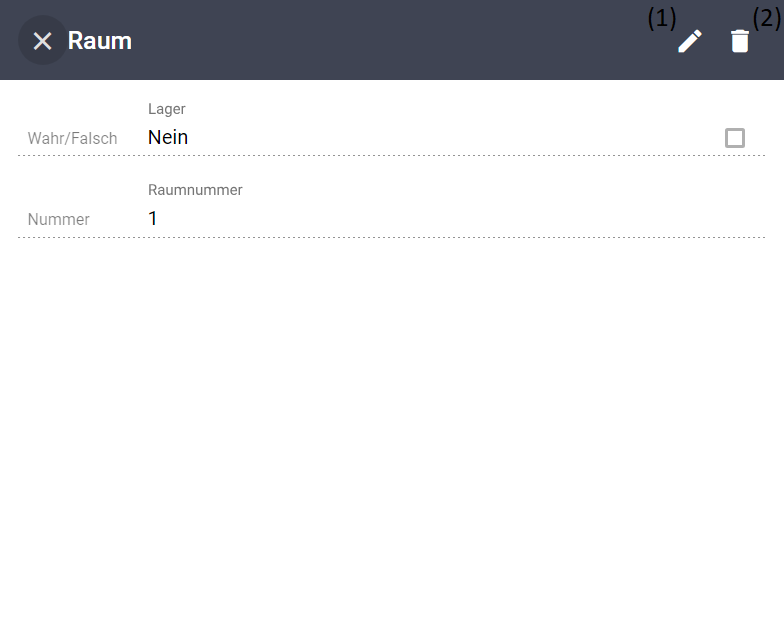
\includegraphics[width=\linewidth]{ObjektInventaredit.png}
	\end{minipage}
	\hfill
	\begin{minipage}{0.4\linewidth}
	\begin{itemize}
		\item[3.] Wählen Sie (1) aus, um das Objekt zu bearbeiten
		\item[4.] Wählen Sie (2) aus, um das Objekt zu löschen
	\end{itemize}
	\end{minipage}\\

	\subsection{Die Sprache ändern}
	\begin{itemize}
		\item[1.] Klicken Sie auf \texttt{DE} oder \texttt{EN} (je nach Standardeinstellung) oben rechts
		\item[2.] Wählen Sie die gewünschte Sprache\\
		\texttt{en} = Englisch\\
		\texttt{de} = Deutsch
	\end{itemize}

	\section{Eigene Daten bearbeiten}
	\begin{itemize}
		\item Klicken Sie auf Ihren Benutzernamen links in der Leiste
	\end{itemize}

	\subsection{Email-Adresse ändern}
		\begin{itemize}
		\item Wählen Sie eine neue gültige Email-Adresse
	\end{itemize}

	\subsection{Passwort ändern}
	\begin{itemize}
		\item[1.] Bestätigen Sie Ihr altes Passwort
		\item[2.] Wählen Sie ein neues Passwort
		\item[3.] Bestätigen Sie das neue Passwort
	\end{itemize}

	\section{Funktionen für den Admin}
	\subsection{eine Benutzerrolle hinzufügen}

	\begin{itemize}
		\item[1.] Klicken Sie auf \glqq{}Benutzerrollen\grqq{}
		\item[2.] Klicken Sie auf \texttt{+} neben der Suchleiste
	\end{itemize}

	\begin{minipage}{0.5\linewidth}
	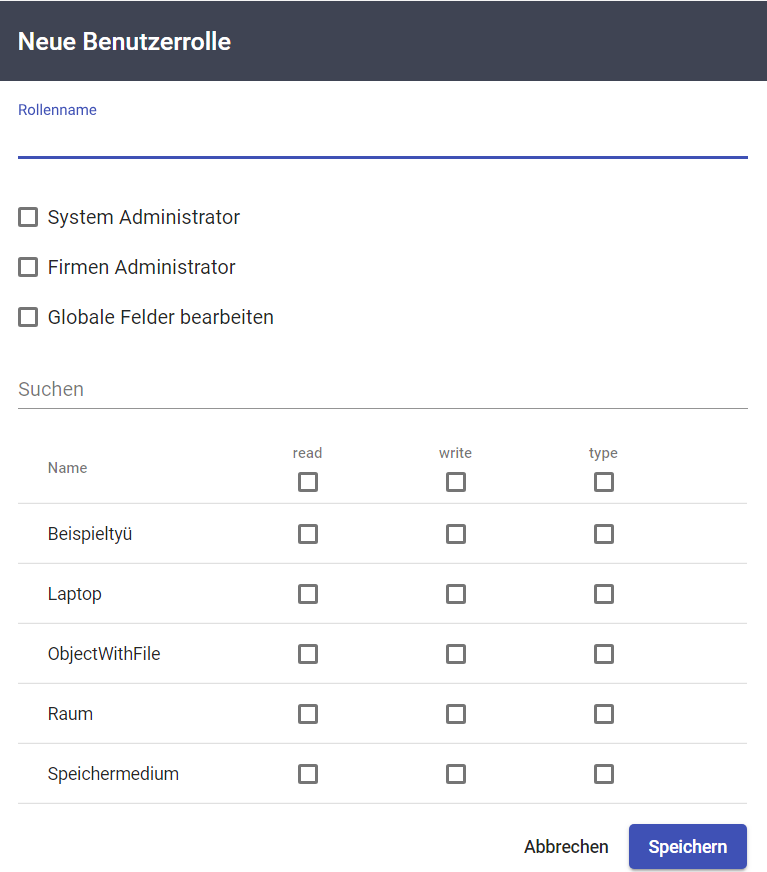
\includegraphics[width=\linewidth]{Rollen.png}
	\end{minipage}
	\hfill
	\begin{minipage}{0.4\linewidth}
	\begin{itemize}
		\item[3.] Wählen Sie einen Namen für die Benutzerrolle aus
		\item[4.] Entscheiden Sie, ob die Benutzerrolle System Administrator, Firmen Administrator ist und ob sie globale Felder bearbeiten können soll\\
		System Administrator = Darf alle Objekttypen, Objekte und Benutzer aller Firmen verwalten\\
		Firmen Administrator = Darf alle Objekttypen, Objekte und Benutzer der Firma, die er angehört, verwalten
		\item[5.] Entscheiden Sie, welche Objekttypen die Benutzerrolle lesen (1) oder bearbeiten (2) kann
	\end{itemize}
	\end{minipage}\\

	\subsection{eine Benutzerrolle bearbeiten}

	\begin{itemize}
		\item[1.] Klicken Sie auf \glqq{}Benutzerrollen\grqq{}
		\item[2.] Klicken Sie auf die Benutzerrolle, die Sie bearbeiten wollen
	\end{itemize}

	\begin{minipage}{0.5\linewidth}
	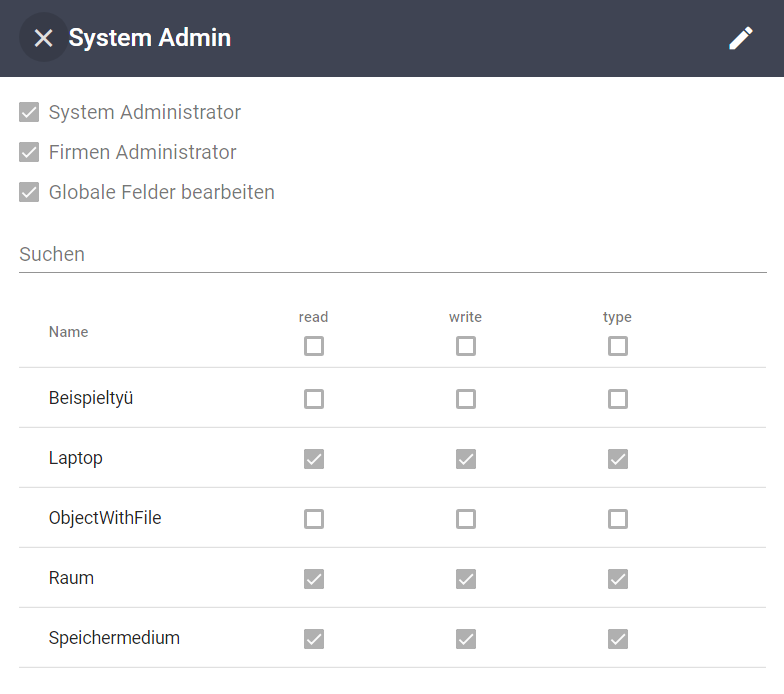
\includegraphics[width=\linewidth]{Rollenedit.png}
	\end{minipage}
	\hfill
	\begin{minipage}{0.4\linewidth}
	\begin{itemize}
		\item[3.] Wählen Sie (1) aus, um die Benutzerrolle zu bearbeiten
		\item[4.] Ändern Sie die gewünschten Rechte
		\item[5.] Klicken Sie auf Speichern
	\end{itemize}
	\end{minipage}\\

	\subsection{Einen Benutzer einer Benutzerrolle hinzufügen}
	
	\begin{itemize}
		\item[1.] Klicken Sie auf \glqq{}Benutzer\grqq{}
		\item[2.] Klicken Sie auf \texttt{+} neben der Suchleiste
	\end{itemize}

	\begin{minipage}{0.5\linewidth}
	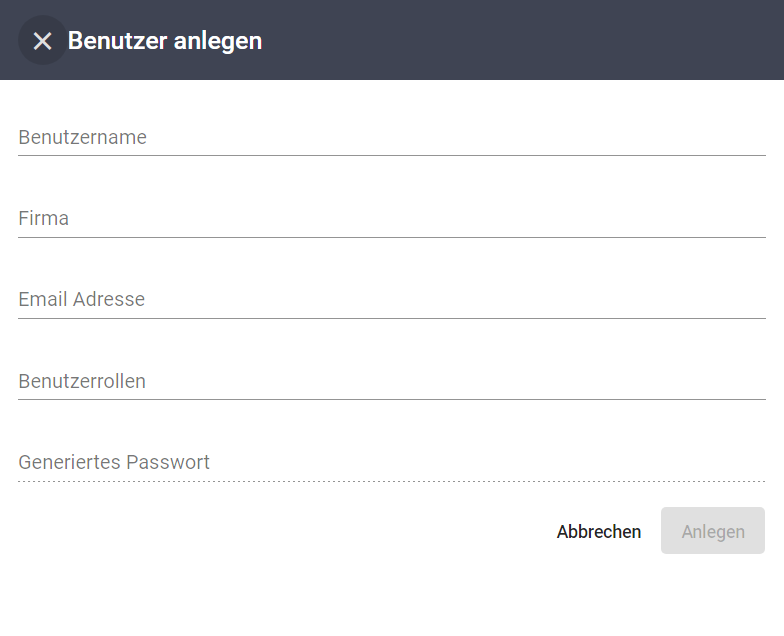
\includegraphics[width=\linewidth]{Benutzer.png}
	\end{minipage}
	\hfill
	\begin{minipage}{0.4\linewidth}
	\begin{itemize}
		\item[3.] Wählen Sie einen Namen für den Benutzer aus
		\item[4.] Entscheiden Sie, welcher Firma der Benutzer angehören soll
		\item[5.] Geben Sie eine gültige Email-Adresse an
		\item[6.] Entscheiden Sie, welche Benutzerrollen der Benutzer haben soll
		\item[7.] Klicken Sie auf Speichern
	\end{itemize}
	\end{minipage}\\

	\subsection{Einen Benutzer bearbeiten}

		\begin{itemize}
		\item[1.] Klicken Sie auf \glqq{}Benutzer\grqq{}
		\item[2.] Klicken Sie auf den Benutzer, den Sie bearbeiten wollen
	\end{itemize}

	\begin{minipage}{0.5\linewidth}
	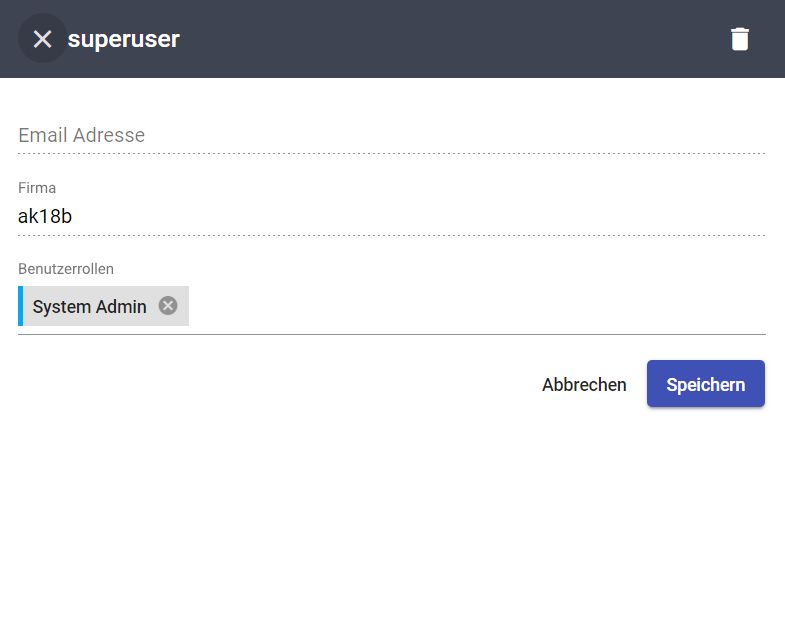
\includegraphics[width=\linewidth]{Benutzeredit.png}
	\end{minipage}
	\hfill
	\begin{minipage}{0.4\linewidth}
	\begin{itemize}
		\item[3.] Ändern Sie die Felder
		\item[4.] Klicken Sie auf Speichern
	\end{itemize}
	\end{minipage}\\

	\subsection{Eine Firma hinzufügen}
	
	\begin{itemize}
		\item[1.] Klicken Sie auf \glqq{}Firmen\grqq{}
		\item[2.] Klicken Sie auf \texttt{+} neben der Suchleiste
		\item[3.] Wählen Sie den Firmennamen
		\item[4.] Klicken Sie auf Speichern
	\end{itemize}

\end{document}